\documentclass[letterpaper,times,twocolumn,10pt]{article}
\usepackage{latex8}
\usepackage{times}
\usepackage{epsfig,ifthen}


%\renewcommand{\topfraction}{0.99}
%\renewcommand{\textfraction}{0.01}
%\renewcommand{\floatpagefraction}{0.99}

\setlength{\topmargin}{0in}
\setlength{\textheight}{9.2in}
\setlength{\textwidth}{7.5in}
\setlength{\topskip}{0in}
\setlength{\footskip}{0in}
\setlength{\headheight}{0in}
\setlength{\headsep}{0in}

%\setlength{\textheight}{9in}
%%\setlength{\columnsep}{0.in}

\def\elide#1{}

\setlength{\oddsidemargin}{-.5in}
\setlength{\evensidemargin}{-.5in}
%\setlength{\textwidth}{6.5in}

%\setlength{\arrayrulewidth}{0.25mm}

%\setlength {\parskip}{1pt plus 0.5pt minus 0.2pt}

\newcommand{\longpage}{\enlargethispage{\baselineskip}}
\newcommand{\shortpage}{\enlargethispage{-\baselineskip}}

\long\def\tbw{\textit{To Be Written}}

%\newenvironment{captiontext}{%
%   \begin{center}%
%     \begin{minipage}{0.9\linewidth}%
%       \renewcommand{\baselinestretch}{0.9}%
%         \small}%
%   {\renewcommand{\baselinestretch}{1.0}%
%      \end{minipage}%
%        \end{center}}


\newenvironment{smitemize}%
  {\begin{list}{$\bullet$}%
     {\setlength{\parsep}{6pt}%
      \setlength{\topsep}{6pt}%
      \setlength{\itemsep}{6pt}}}%
  {\end{list}}

\makeatletter
\long\def\unmarkedfootnote#1{{\long\def\@makefntext##1{##1}\footnotetext{#1}}}
\makeatother

\raggedbottom

%----------------------------------------------------------------


\begin{document}

\twocolumn[%

\centerline{\Large \sffamily \bfseries { eFlux: Simple Automatic Adaptation for Environmentally Powered Devices}}

\medskip

%\title{eFlux: Simple Automatic Adaptation for Environmentally Powered Devices
%\date{}
%}
%\author{
\centerline{
\begin{tabular}{ccccc}
{\bf Jacob Sorber} & {\bf Alexander Kostadinov} & {\bf Matt Brennan} & {\bf Mark Corner} & {\bf Emery Berger}\\
\multicolumn{5}{c}{Department of Computer Science}\\
\multicolumn{5}{c}{University of Massachusetts, Amherst, MA}\\
\multicolumn{5}{c}{\{sorber, akostadi, mbrennan, mcorner, emery\}@cs.umass.edu}
\end{tabular}
}
\bigskip
\bigskip
]
%}
\thispagestyle{empty}
%\maketitle
{\small
\section*{Introduction}

Energy management is a critical problem in designing mobile computing
systems, especially when those systems depend on harvesting energy
from environmental sources, such as solar or wind.  Environmental
sources are highly variable and difficult to predict, which is often
complicated further by device mobility.  In this demo, we present a
simple approach for developing energy-aware applications using a
high-level data flow oriented coordination language.  This language,
eFlux, is an extension of the Flux~\cite{flux} coordination language,
which provides a simple interface for specifying an energy adaptation
policy, which can then be implemented automatically by the underlying
runtime system.  This approach allows a system designer to change the
underlying adaptation algorithms (e.g. energy source prediction)
without modifying the application.  Also, the data flow programming
style of Flux simplifies program profiling and performance prediction.

In this demo, we will present our experience, to date, using eFlux,
including both working system and simulation results.  We will
also demonstrate an energy-aware GPS tracking device for tracking
threatened Wood Turtles in Western Massachusetts.  


\section*{Wildlife Tracking}



The motivation for our research comes, in part, from the efforts of
conservation biologists to protect threatened turtles.  The Wood
Turtle~(Clemmys~insculpta), shown in Figure~\ref{fig:turtle}, is found
throughout the Northeast and Great Lakes regions and into Canada.
They live primarily in and along streams; however, they are also
terrestrial for about 4~months of the year.  Wood Turtles are of
particular interest since their numbers are rapidly declining due to
habitat destruction and highway mortality~\cite{turtlesernst}.
Unfortunately, conservation efforts have been hindered by a general
lack of data due to current tracking methods.  Researchers currently
track turtles manually using radio telemetry and are limited to taking
a single location fix every 2-3~days for each animal being studied.
The turtles often travel up to 1~kilometer between fixes and practical
concerns preclude the collection of location information at night.  In
order to more accurately understand how these turtles behave and use
their habitat, new tracking methods are required to collect data at
finer granularity.  


Recent advances in sensing platforms make it possible to use more
sophisticated sensors, such as a GPS receiver, to collect more
frequent movement information.  A sensor platform such as a Crossbow
Mica2Dot, a GPS receiver, a flexible solar panel, and
a small 250mAhr lithium polymer battery are within the acceptable
weight and size requirements, for studying these animals; however,
energy management remains a significant concern.  A typical GPS
receiver will completely drain a 250mAhr battery in less than 2 hours,
which necessitates carefully selecting an appropriate duty~cycle based
on the energy stored in the battery as well as the expectation of
energy from its solar panel.  Due to the high variance of solar
radiation and the unknown mobility patterns of the individual turtles,
it is necessary for us to dynamically adjust device behavior during
operation.  Our goal is to provide a simple programming system that
meets these needs.




%\begin{figure}[t]
%\centering
%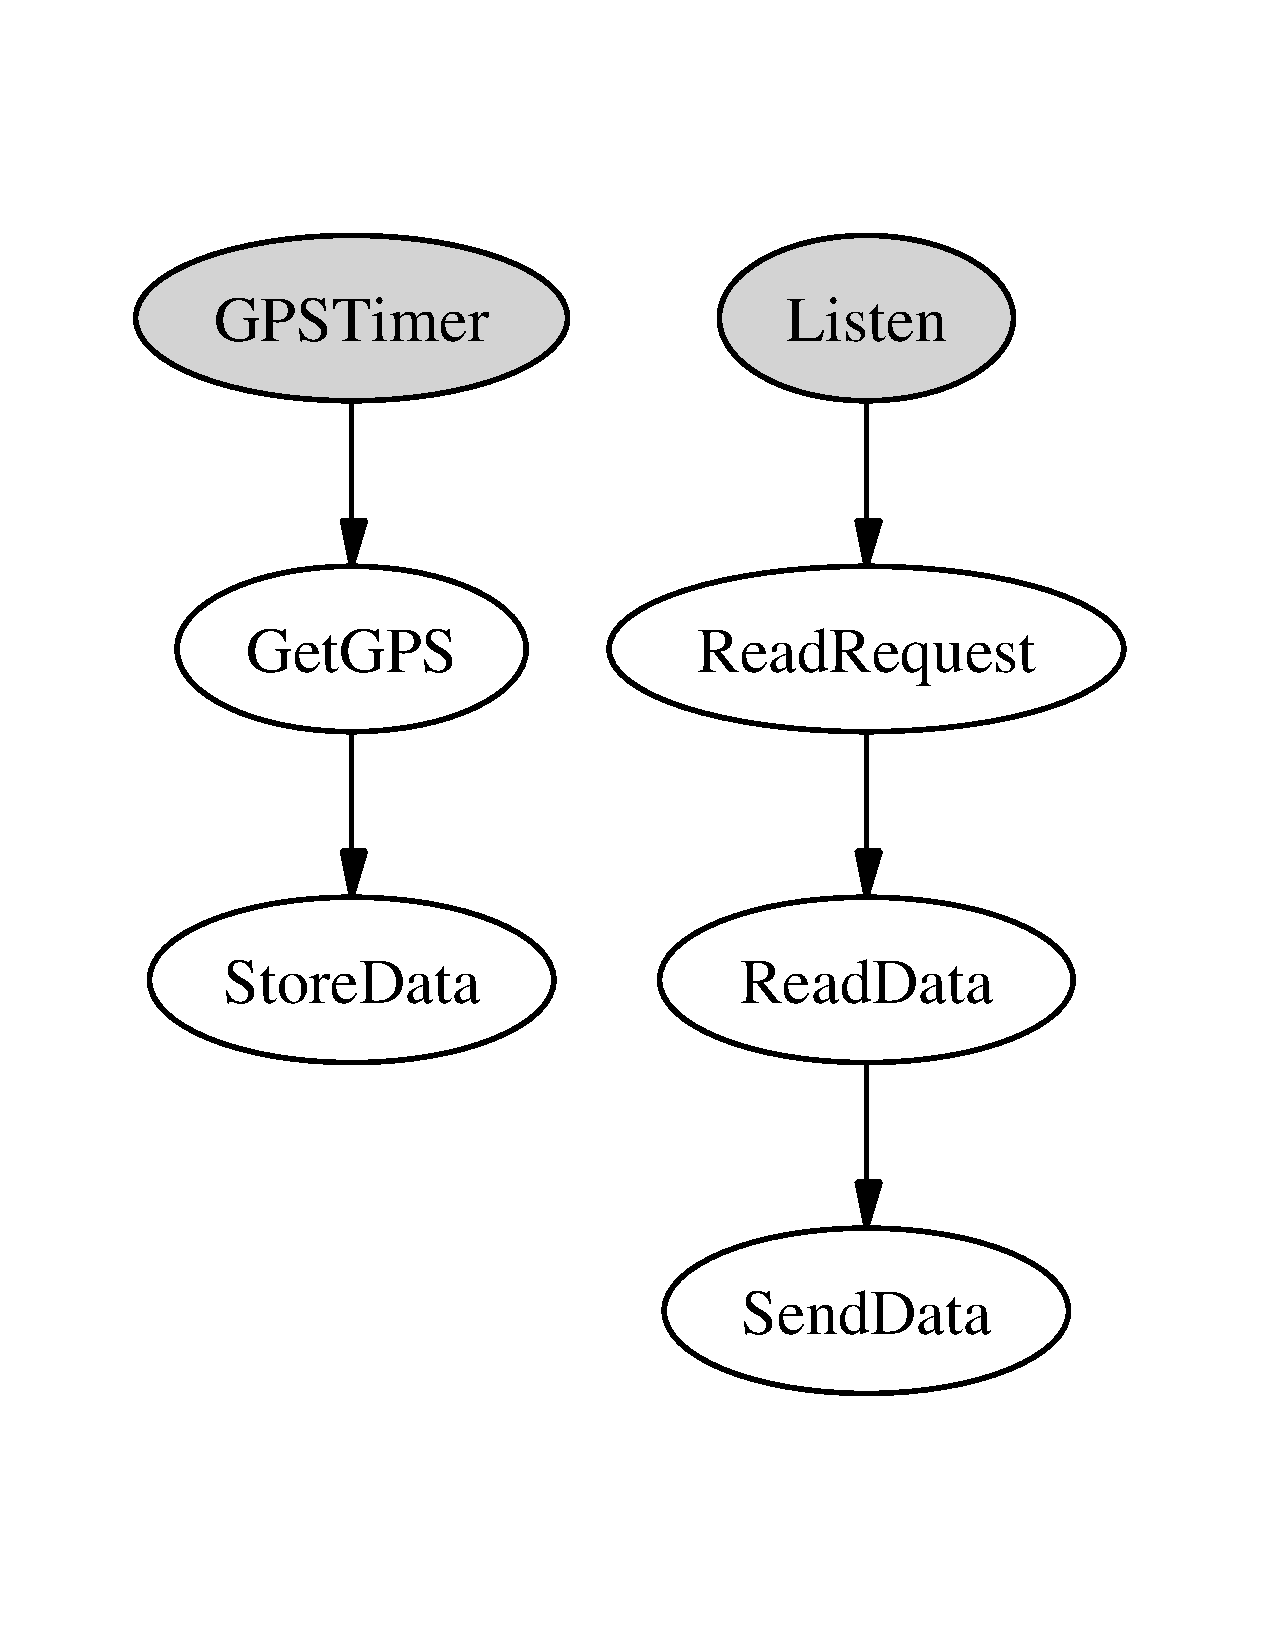
\includegraphics[width=3in]{fig/fluxg2}
%\caption{A sample Flux flow graph}
%\label{fig:graph}
%\end{figure}

\section*{Language Description}

\begin{figure}[t]
\centering
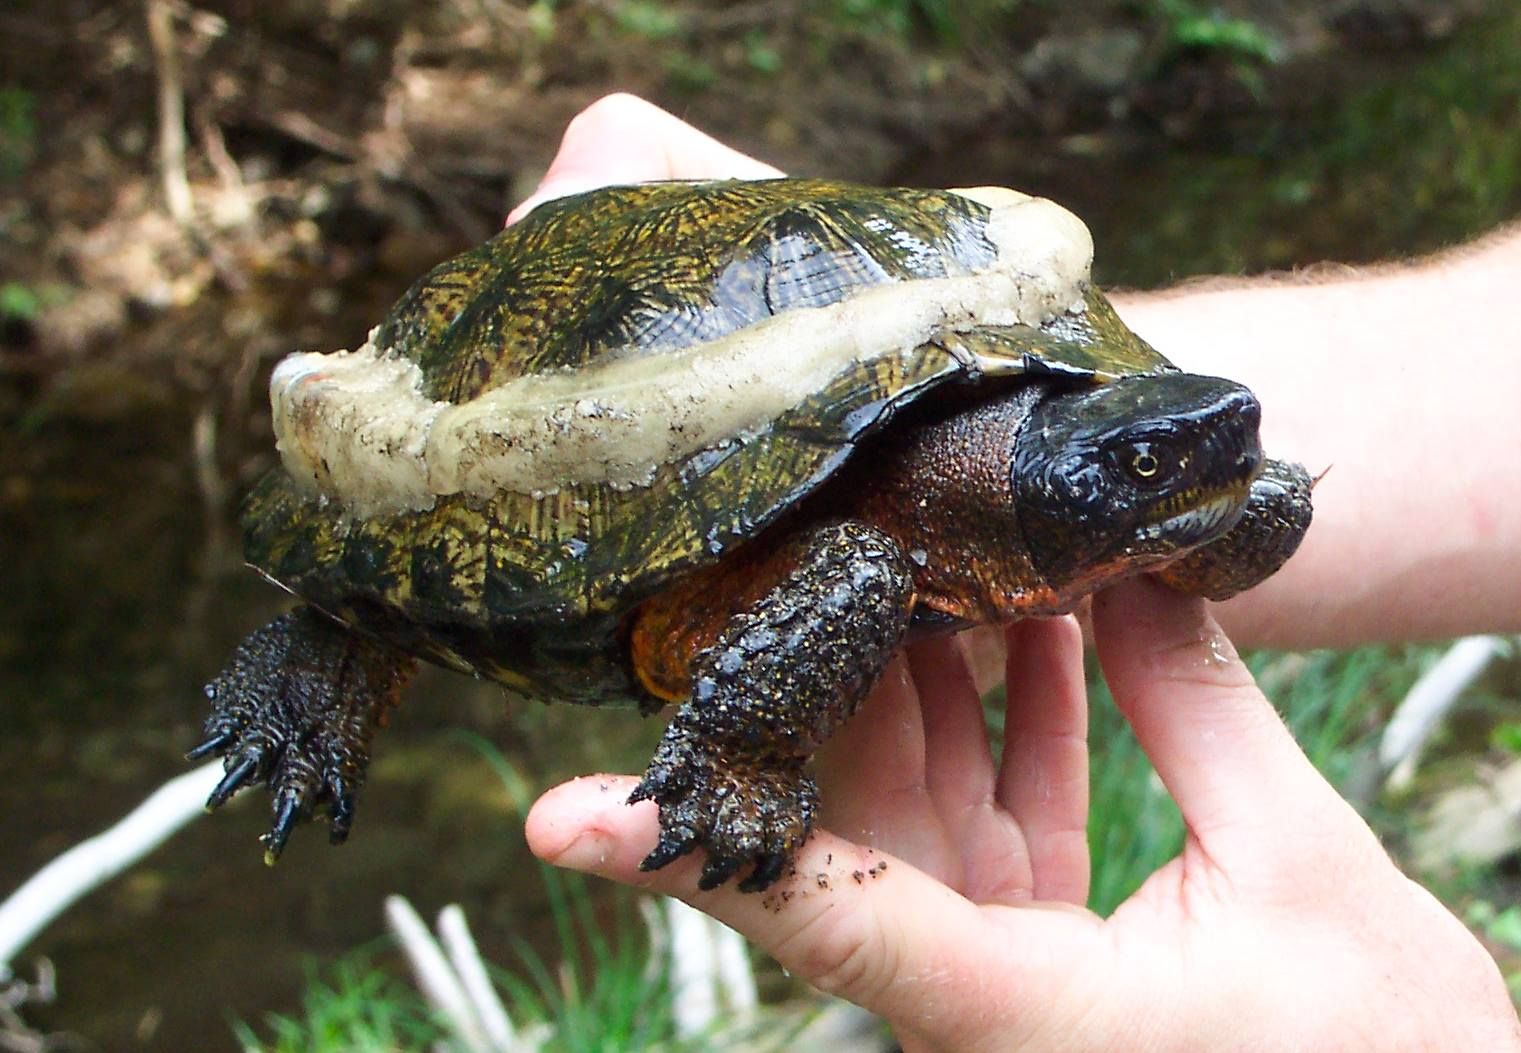
\includegraphics[width=2.5in]{fig/turtle}
\caption{Wood Turtle with radio transmitter attached}
\label{fig:turtle}
\end{figure}

The data-flow oriented programming style used in the Flux\cite{flux}
language has many similarities with the programming style used in many
sensor systems.  A Flux program is a directed acyclic graph(DAG) that
describes how data and control flow from event sources through
computational tasks.  While this program style was originally
designed to support the programming needs of high-performance servers,
network embedded sensor applications also typically consist of a
sequence of tasks that are performed in response to an event, such as
an expired timer or the arrival of a network message.


In this demonstration, we present eFlux (embedded Flux), which extends
Flux to include an application adaptation policy which describes an
ordering of behavior adjustments, which include alternate control
paths and adjustable timers.  We will present an eFlux compiler and
runtime system that implements this policy, by profiling the energy
cost and frequency of individual execution paths and determining an
appropriate operating state.  

\bibliographystyle{acm}
\bibliography{eflux}

}
\end{document}

